\documentclass[a4paper,fleqn]{article} %Options in documentclass should be set to a4paper and fleqn.
\usepackage{modsim}
\usepackage{times}
\usepackage{psfrag}
 \usepackage{pstricks}
 %\usepackage{auto-pst-pdf}
\usepackage{pstool}
\usepackage{natbib} %The three packages modsim, times and natbib are required.
\usepackage{amsmath, amssymb, amsthm} %Also recommend the standard AMS LaTeX maths packages.

\newcommand\solidrule[1][0.25cm]{\rule[0.5ex]{#1}{1pt}}
\newcommand\dashedrule{\mbox{%
		\solidrule[2mm]\hspace{2mm}\solidrule[2mm]}}
\pagestyle{MODSIMheadings} %Calling the MODSIM Headings format
\MODSIMhead{J. Pitt {\it et al.}, Importance of Dispersion for Shoaling Waves} %This is the content of the headings in all pages (except the first page). The format should be author, title of paper. If the title is too long, then use ... at the end. If more than two authors, then please use the "et al." format with et al. in italic, for example A. Author {\it et al.}, Title of the paper.

% Define any other command or required packages below:
%%%%%%%%%%%%%%%%%%%%%%%%%%%%%%%%%%%%%%%%%%%%%%%%%%%%%%%%%%%%%%%%%%%%%%%%%%%%%%%%%%%%%%%%%%%%%%%%%%%%%%%%%%%
\usepackage{rotating}
\usepackage{amsbsy,enumerate}
\usepackage{graphicx}
\usepackage{ccaption}
\newcommand{\ve}{\varepsilon}
\newcommand{\sigmah}{\hat{\sigma}}
\newcommand{\sigmab}{\bar{\sigma}}
\newcommand{\R}{\mathbb{R}}
\newcommand{\Z}{\mathbb{Z}}
\newcommand{\E}{\mathbb{E}}
\newcommand{\Tbar}{\bar{T}}
\newcommand{\Thetabf}{\mathbf{\Theta}}
\newcommand{\Xbf}{\mathbf{X}}
\newcommand{\xbf}{\mathbf{x}}
\newcommand{\Ybf}{\mathbf{Y}}
\newcommand{\ybf}{\mathbf{y}}
\newcommand{\Ubf}{\mathbf{U}}
\newcommand{\Fbf}{\mathbf{F}}
\newcommand{\fbf}{\mathbf{f}}
\newcommand{\Pbf}{\mathbf{P}}
\newcommand{\Pbfbar}{\bar{\mathbf{P}}}
\newcommand{\Sb}{\bar{S}^{\nu}}
\newcommand{\Snuib}{\tilde{S}^\nu _i}
\newcommand{\Snui}{S^\nu _i}
\newcommand{\sigmanui}{\sigma ^\nu_i}
\newtheorem{lemma}{Lemma}
\newtheorem{corollary}{Corollary}
\newtheorem{assumption}{Assumption}
\newtheorem{theorem}{Theorem}
\newtheorem{remark}{Remark}
\newtheorem{definition}{Definition}
\newtheorem{cce}{Assumption CCE}
\newtheorem{proposition}{Proposition}
%% The next four lines create the correct format for Figure and Table captions. They require the package "ccaption".
\makeatletter
\renewcommand{\fnum@figure}[1]{\textbf{\figurename~\thefigure}. }
\renewcommand{\fnum@table}[1]{\textbf{\tablename~\thetable}. }
\makeatother

%%%%%%%%%%%%%%%%%%%%%%%%%%%%%%%%%%%%%%%%%%%%%%%%%%%%%%%%%%%%%%%%%%%%%%%%%%%%%%%%%%%%%%%%%%%%%%%%%%%%%%%%%%%

\begin{document}
% Defining Front matter.

\title{Importance of Dispersion for Shoaling Waves}
\author{\underline{J. Pitt} \address[ANU]{\it{Mathematical Sciences Institute, Australian National University, Canberra, ACT 0200, Australia}}, C. Zoppou \addressmark[ANU], S.G Roberts \addressmark[ANU]}


\email{jordan.pitt@anu.edu.au} %Email address of the presenting author only.

\date{June 2017}

%Keywords should be separated by commas and listed in Sentence case (first keyword with capital first letter and remaining keywords in lower case).
\begin{keyword}
	Tsunamis, shoaling waves, dispersion, models

\end{keyword}

\begin{abstract}
	Flooding has been responsible for some of the deadliest natural disasters in human history because, our densest areas of population occur along rivers and/or close to the coast. The worst of these in living memory was the 2004 Indian Ocean tsunami, which sparked much of the current research we do into inundation at the ANU via the ANUGA software,which was developed in collaboration with Geoscience Australia. The interaction of waves with bathymetry and particularly the shoaling of waves plays a central role in modelling the inundation caused by a tsunami. Current industrial models for tsunami inundation such as ANUGA utilize the non-dispersive shallow water wave equations. Current research into tsunami inundation includes building numerical models based on dispersive equations, such as the Serre equations. Dispersive equations allow waves of different frequencies to travel at different speeds thereby capturing
	more fluid behaviour. They are theoretically a better choice as the basis for inundation models. However, these methods are computationally expensive and the detailed behaviour is not always significant. When the water depth is large compared to the wave height, the propagation of a wave is not strongly
	influenced by different frequency speeds associated with dispersion waves. In this case the numerical results for the non-dispersive and dispersive equations are similar. The behaviour of the waves in deep water is well understood, this is not the case for the behaviour of waves in the nearshore. We investigate these waves by numerically modelling experimental data of the propagation of waves over a submerged trapezoidal bar using both the non-dispersive 
	shallow water wave equations and the dispersive Serre equations. Comparing the results from these simulations provides an opportunity to assess the importance of dispersion for the propagation of waves over a submerged bar and shoaling waves on a linear beach.

\end{abstract} %Abstract should NOT extend beyond the first page.

\maketitle

\section{INTRODUCTION}


%--------------------------------------------------------------------------------
\section{Periodic Wave Over a Submerged Bar}
\label{Oscillatory Wave Over a Submerged Bar}
%--------------------------------------------------------------------------------
\cite{Beji-Battjes-1994} conducted a series of experiments where waves travel over a submerged trapezoidal bar. Their wave tank was $37.7$m in length, $0.8$m wide and $0.75$m high with a constant water stage of $0.4$m. The bed had the following profile; $(x,z_b) = [$($0$m,$0$m), ($6$m,$0$m), ($12$m,$0.3$m), ($14$m,$0.3$m), ($17$m,$0$m), ($18.95$m,$0$m), ($28.95$m,$0.4$m)$]$. Waves were generated by a wave maker located at $x=0$m, and were absorbed downstream by a $3$m long gravel beach, with a slope of $1:25$. There were seven wave gauges that recorded the depth of water over time at the following locations; WG1: $5.7$m, WG2: $10.5$m, WG3: $12.5$m, WG4: $13.5$m, WG5: $14.5$m, WG6: $15.7$m and WG7: $17.3$m. 

In this paper we focus on one of these experiments that investigated periodic non-breaking sinusoidal waves with low frequency propagating over the bar. These waves had a period of $T = 2$s, a wavelength of $\lambda \approx 3.69$m and an amplitude of $A = 0.01$m. These waves travel without deformation towards the bar. The waves then steepen as they travel up the front slope of the bar due to shoaling. On the horizontal top of the bar higher harmonic waves are slowly released. This release of waves is then accelerated as the waves travel down slope. After the bar the waves reach an equilibrium and again begin to travel without deformation. Although bars do occur throughout the worlds oceans, in the context of tsunami modelling we are more interested in the behaviour of waves on the front slope region and the horizontal top of the bar and so we focus on wave gauges $1$ through $4$. 

We have numerically simulated this experiment using a numerical method for the Serre equations by \cite{Zoppou-etal-2017} and the numerical modelling software ANUGA for the shallow water wave equations []. The results for the Serre equations are presented in Figure \ref{fig:Baji_1994-SL_simulation} and the results for the shallow water wave equations are presented in Figure []. 

\begin{figure}[htb]
	\centering
	\begin{tabular}{ccc}
		\begin{psfrags}%
			\psfragscanon%
			%
			% text strings:
			\psfrag{s03}[t][t][2.0]{\color[rgb]{0,0,0}\setlength{\tabcolsep}{0pt}\begin{tabular}{c}$t$(s)\end{tabular}}%
			\psfrag{s04}[b][b][2.0]{\color[rgb]{0,0,0}\setlength{\tabcolsep}{0pt}\begin{tabular}{c}$h$(cm)\end{tabular}}%
			%
			% xticklabels:
			\psfrag{x01}[t][t][1.5]{50}%
			\psfrag{x02}[t][t][1.5]{51}%
			\psfrag{x03}[t][t][1.5]{52}%
			\psfrag{x04}[t][t][1.5]{53}%
			\psfrag{x05}[t][t][1.5]{54}%
			\psfrag{x06}[t][t][1.5]{55}%
			\psfrag{x07}[t][t][1.5]{56}%
			\psfrag{x08}[t][t][1.5]{57}%
			\psfrag{x09}[t][t][1.5]{58}%
			%
			% yticklabels:
			\psfrag{v01}[r][r][1.5]{-2}%
			\psfrag{v02}[r][r][1.5]{-1}%
			\psfrag{v03}[r][r][1.5]{ 0}%
			\psfrag{v04}[r][r][1.5]{ 1}%
			\psfrag{v05}[r][r][1.5]{ 2}%
			\psfrag{v06}[r][r][1.5]{ 3}%
			%
			% Figure:
			\resizebox{5cm}{!}{\includegraphics{Beji-1994-SL-WG1.eps}}%
		\end{psfrags}%
		& &
		\begin{psfrags}%
			\psfragscanon%
			%
			% text strings:
			\psfrag{s03}[t][t][2.0]{\color[rgb]{0,0,0}\setlength{\tabcolsep}{0pt}\begin{tabular}{c}$t$(s)\end{tabular}}%
			\psfrag{s04}[b][b][2.0]{\color[rgb]{0,0,0}\setlength{\tabcolsep}{0pt}\begin{tabular}{c}$h$(cm)\end{tabular}}%
			%
			% xticklabels:
			\psfrag{x01}[t][t][1.5]{50}%
			\psfrag{x02}[t][t][1.5]{51}%
			\psfrag{x03}[t][t][1.5]{52}%
			\psfrag{x04}[t][t][1.5]{53}%
			\psfrag{x05}[t][t][1.5]{54}%
			\psfrag{x06}[t][t][1.5]{55}%
			\psfrag{x07}[t][t][1.5]{56}%
			\psfrag{x08}[t][t][1.5]{57}%
			\psfrag{x09}[t][t][1.5]{58}%
			%
			% yticklabels:
			\psfrag{v01}[r][r][1.5]{-2}%
			\psfrag{v02}[r][r][1.5]{-1}%
			\psfrag{v03}[r][r][1.5]{ 0}%
			\psfrag{v04}[r][r][1.5]{ 1}%
			\psfrag{v05}[r][r][1.5]{ 2}%
			\psfrag{v06}[r][r][1.5]{ 3}%
			%
			%
			% Figure:
			\resizebox{5cm}{!}{\includegraphics{Beji-1994-SL-WG2.eps}}%
		\end{psfrags}%
		\\
		WG1 & & WG2  \\ \\
		\begin{psfrags}%
			\psfragscanon%
			%
			% text strings:
			\psfrag{s03}[t][t][2.0]{\color[rgb]{0,0,0}\setlength{\tabcolsep}{0pt}\begin{tabular}{c}$t$(s)\end{tabular}}%
			\psfrag{s04}[b][b][2.0]{\color[rgb]{0,0,0}\setlength{\tabcolsep}{0pt}\begin{tabular}{c}$h$(cm)\end{tabular}}%
			%
			% xticklabels:
			\psfrag{x01}[t][t][1.5]{50}%
			\psfrag{x02}[t][t][1.5]{51}%
			\psfrag{x03}[t][t][1.5]{52}%
			\psfrag{x04}[t][t][1.5]{53}%
			\psfrag{x05}[t][t][1.5]{54}%
			\psfrag{x06}[t][t][1.5]{55}%
			\psfrag{x07}[t][t][1.5]{56}%
			\psfrag{x08}[t][t][1.5]{57}%
			\psfrag{x09}[t][t][1.5]{58}%
			%
			% yticklabels:
			\psfrag{v01}[r][r][1.5]{-2}%
			\psfrag{v02}[r][r][1.5]{-1}%
			\psfrag{v03}[r][r][1.5]{ 0}%
			\psfrag{v04}[r][r][1.5]{ 1}%
			\psfrag{v05}[r][r][1.5]{ 2}%
			\psfrag{v06}[r][r][1.5]{ 3}%
			%
			%
			% Figure:
			\resizebox{5cm}{!}{\includegraphics{Beji-1994-SL-WG3.eps}}%
		\end{psfrags}%
		& &
		\begin{psfrags}%
			\psfragscanon%
			%
			% text strings:
			\psfrag{s03}[t][t][2.0]{\color[rgb]{0,0,0}\setlength{\tabcolsep}{0pt}\begin{tabular}{c}$t$(s)\end{tabular}}%
			\psfrag{s04}[b][b][2.0]{\color[rgb]{0,0,0}\setlength{\tabcolsep}{0pt}\begin{tabular}{c}$h$(cm)\end{tabular}}%
			%
			\psfrag{x01}[t][t][1.5]{50}%
			\psfrag{x02}[t][t][1.5]{51}%
			\psfrag{x03}[t][t][1.5]{52}%
			\psfrag{x04}[t][t][1.5]{53}%
			\psfrag{x05}[t][t][1.5]{54}%
			\psfrag{x06}[t][t][1.5]{55}%
			\psfrag{x07}[t][t][1.5]{56}%
			\psfrag{x08}[t][t][1.5]{57}%
			\psfrag{x09}[t][t][1.5]{58}%
			%
			% yticklabels:
			\psfrag{v01}[r][r][1.5]{-2}%
			\psfrag{v02}[r][r][1.5]{-1}%
			\psfrag{v03}[r][r][1.5]{ 0}%
			\psfrag{v04}[r][r][1.5]{ 1}%
			\psfrag{v05}[r][r][1.5]{ 2}%
			\psfrag{v06}[r][r][1.5]{ 3}%
			%
			%
			% Figure:
			\resizebox{5cm}{!}{\includegraphics{Beji-1994-SL-WG4.eps}}%
		\end{psfrags}%
		\\
		WG3 & & WG4 \\ \\

		\end{tabular}
		\caption{Simulated and observed water surface at several gauges for a sinusoidal wave with period, $T = 2$s traveling over a submerged reef conducted by \cite{Beji-Battjes-1994}.}
		\label{fig:Baji_1994-SL_simulation}
	\end{figure}
	
\begin{figure}
	\centering
	\resizebox{6cm}{!}{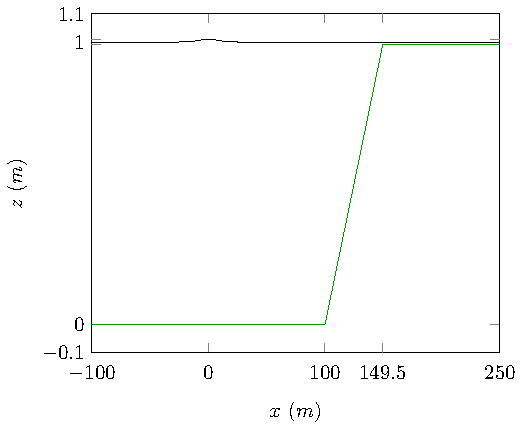
\includegraphics{solitonslopeSerre1.pdf}}
	\\
	\hspace{10 mm}$t= 0s$
	\\ 
	\begin{tabular}{ccc}
	\resizebox{5cm}{!}{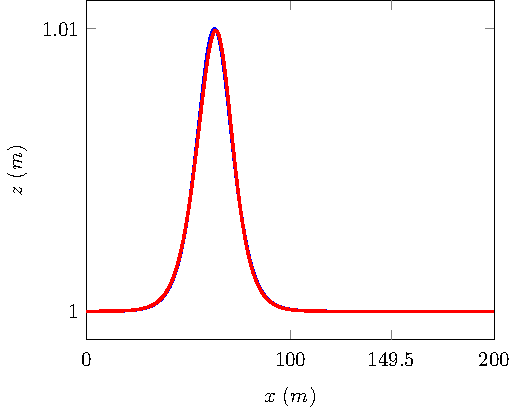
\includegraphics{solitonslopeSerre2.pdf}} & & \resizebox{5cm}{!}{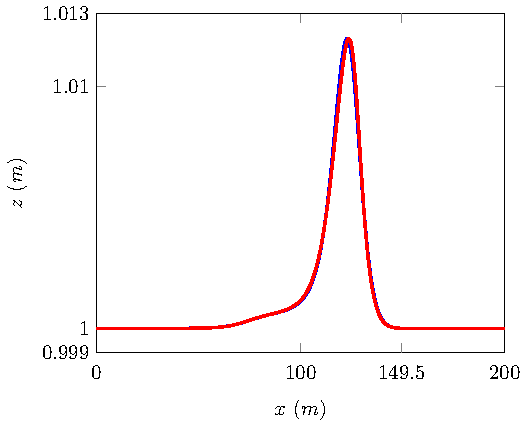
\includegraphics{solitonslopeSerre3.pdf}}  \\
	\hspace{5 mm} $t= 20s$ & & \hspace{5 mm}$t= 40s$ \\
	\resizebox{5cm}{!}{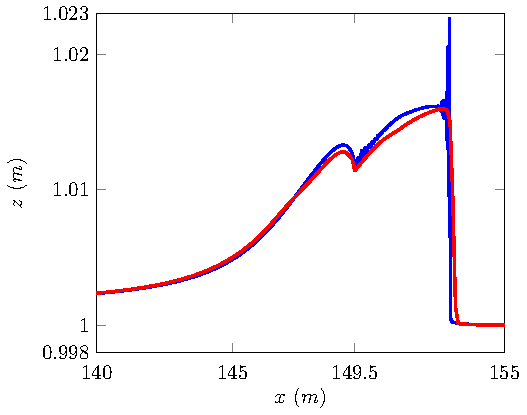
\includegraphics{solitonslopeSerre4.pdf}} && 
	 \resizebox{5cm}{!}{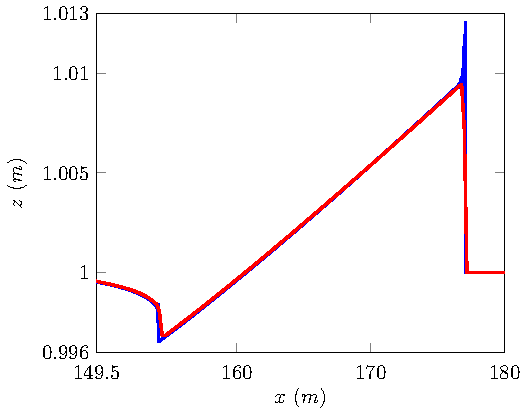
\includegraphics{solitonslopeSerre5.pdf}}  \\
	 \hspace{5 mm} $t= 50s$ & & \hspace{5 mm} $t= 100s$ \\
		
		
	\end{tabular}
	\caption{The stage ({\color{blue} \solidrule}) and bed ({\color{green!60!black} \solidrule}) from the numerical solution of the Serre equations for the soliton travelling over a slope, at different times.}
	\label{fig:allstructs}
\end{figure}
	
\bibliographystyle{chicago} %use chicago style of referencing.
\bibliography{DamBreak}
\end{document}
